% CREATED BY MAGNUS GUSTAVER, 2020
\chapter{Theory}

This chapter describes the theory behind the method of the project. It does this by describing the programs and hardware that has been used during the development of the Autobike, or in the final result. Note that the hardware presented below does not include all components of the Autobike, but instead only a selection which were deemed relevant to this project and report.

\section{LabVIEW}
LabVIEW is a graphical programming environment used to "develop automated research, validation, and production test systems" \cite{NationalInstruments2022WhatLabVIEW}. The language used in LabVIEW is called G, and programming is performed by connecting blocks called VI's (virtual instruments) or nodes using wires \cite{Andrade1998SoftwareTM}. These VI's can either be a "sub-VI" written in G, or primitives built into G.

National Instruments, the developers behind LabVIEW, describes the benefits of the G programming language as being easy for engineers and scientists to learn, as well as being more intuitive to debug than text based languages \cite{NationalInstruments2022BenefitsLabVIEW}. They also describe LabVIEW as allowing "automatic parallelization", since it is a dataflow language, in contrast to sequential languages like C where this is not possible. Figure \ref{fig:lab-example} below shows an example of a LabVIEW program.

\begin{figure}[H]
    \centering
    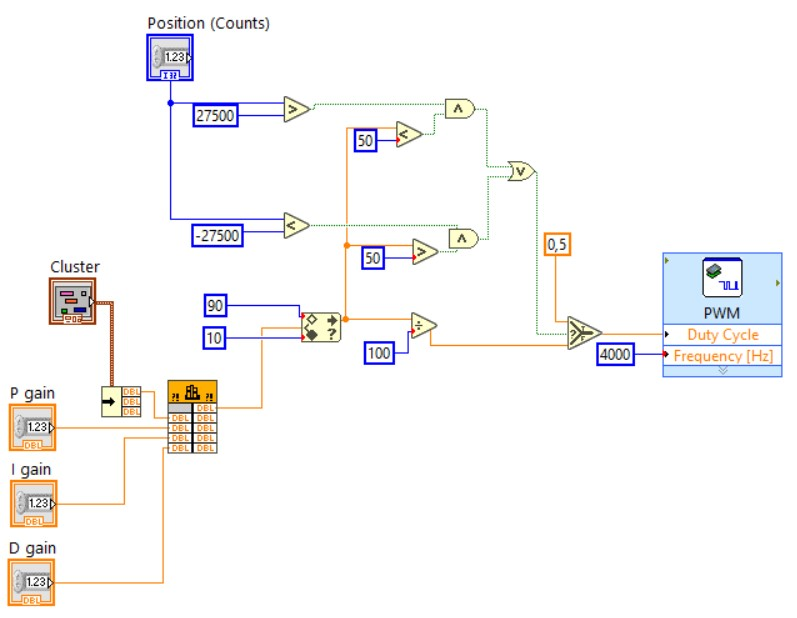
\includegraphics[width=6cm]{figure/labview_example.jpg}
    \caption{Example of a LabVIEW program.}
    \label{fig:lab-example}
\end{figure}

\subsection{Integration With Text Based Languages}
Certain parts of a LabVIEW program may not be not suited for development in G, instead a text based language can be used and integrated into LabVIEW \cite{NationalInstruments2022BenefitsLabVIEW}. The integration can be either done by using the \textit{Formula Node} to write code with a syntax similar to C, or using the \textit{Call Library Function Node} to call a DLL (Dynamic-link library) or a shared library function \cite{Nationalinstruments2018CallNode}. The node takes in function parameters as specified in the node's settings, and uses their values when calling the specified function. When the called function completes, its value is returned and can be used by other parts of the LabVIEW program.

To be able to call a function using the Call Library Function Node the code must be compiled to either a DLL, or a shared library (a file with a .so filename extension) if using a Linux based target \cite{NationalInstruments2021CreatingTarget}. This library or DLL must then be uploaded to the target using for example SFTP (SSH file transfer protocol). If the target is Linux based the library should be uploaded to the \texttt{/usr/local/lib} directory. The name of the .so file should then be specified in LabVIEW inside the settings of the Call Library Function Node.

\section{MyRIO-1900}
The MyRIO-1900 is a device that combines multiple components such as an ARM processor, an FPGA (field programmable gate array)\footnote{An FPGA is an integrated circuit that consists of an array of logic gates, which can be configured by the user to create a specific hardware architecture \cite{Trochimiuk2021FPGAUsed}.}, as well as both analog and digital I/O (input / output) lines to help "students and educators complete real engineering projects in one semester" \cite{NationalInstruments2022MyRIO-1900}. The RIO architecture that the myRIO uses combines a processor with the I/O of the device via an FPGA \cite{NationalInstruments2020TheInnovation, NationalInstruments2022FromNI}. In the RIO architecture, the FPGA is connected directly to the I/O and is used to offload critical and intensive tasks from the processor \cite{NationalInstruments2022FromNI}. It also makes high throughput tasks that run on the FPGA more deterministic than if they had run on the processor.

\section{ESCON Motor Controller}
The ability to steer the front wheel of the bike is made possible by a the so called steering motor. The motor controller for the steering motor is an ESCON 50/5 designed by Maxon. This motor controller is a "PWM servo controller", which means it controls motors using Pulse Width Modulation (PWM). The PWM duty cycle range of the controller, meaning the range between which values the duty cycle can be varied, is 10\% to 90\% \cite{Maxon2021ESCONReference}.

\section{Steering Motor Encoder}
To measure the position of the steering motor, or how far the front wheel has been rotated, an encoder of the model HEDS-5540\#A11 is used. The encoder translates rotational motion into a digital signal by using a codewheel that interrupts a light beam when it spins \cite{AvagoTechnologies2014HEDM-55xx/560xHEDS-55xx/56xx}. The encoder outputs a waveform signal with a resolution of 500 counts per revolution.

\section{Inertial Measurement Unit (IMU)}
The bike features an Inertial Measurement Unit, or IMU, the specific model of IMU used is a Pmod NAV designed by Digilent. This device features an accelerometer and a gyroscope, as well as a magnetometer and a barometer, the latter pair of which are not used in this project. Both the accelerometer and gyroscope makes measurements in relation to the 3 Cartesian coordinate axes \cite{Digilent2017PmodManual}. The units of the given measurements are \textit{g} (circa $9.81 m/s^2$), and \textit{dps} (degrees per second) for the accelerometer and gyroscope respectively; these measurements are given separately for each of the three axes \cite{STMicroelectronics2015INEMOMagnetometer}.

\section{UART Communication}
Universal asynchronous receiver-transmitter, abbreviated to UART, is a device-to-device hardware communication protocol \cite{GraceLegaspi2020UART:Receiver/Transmitter}. UART is used to transmit and receive serial data between two devices, this is achieved with only two wires for the transmitting and receiving ends. Each of the UART devices has two signals named transmitter (Tx), and receiver (Rx); the transmitter of one device should be connected to the receiver of the other, and vice versa.

The UART interface is, as its name implies, asynchronous, meaning it does not use a clock signal for synchronization. Instead a bitstream is generated by the transmitter, which is sampled by the receiver; synchronization is accomplished by using the same baud rate on both of the devices.
The baud rate is the rate at which the information from the transmitter is sent.

Information is transferred in the form of a packet. The packet includes a start bit, the data frame, an eventual parity bit, and finally one or two stop bits. The start and stop bits indicate the borders of a packet, meaning its start and end. The data frame contains the actual data which is transferred, it has a maximum length of 9 bits if no parity bit is used, otherwise the maximum length is 8 bits. The parity bits can optionally be used to tell if the data frame has been changed during the transmission.

\section{VESC}
The VESC is a controller for brushless DC motors, also known as an ESC (electronic speed controller) \cite{Vedder2014AESC}. Both the hardware and firmware are open source, and available on GitHub\footnote{The hardware and firmware can be found on GitHub at \url{https://github.com/vedderb/bldc-hardware} and \url{https://github.com/vedderb/bldc respectivly.}}. Communication with the ESC can be done using either a PPM signal, analog, UART, I2C, USB or CAN \cite{Vedder2016VESCESC}.

Vedder describes in \cite{Vedder2015CommunicatingUART} that when communicating with the controller using UART, each packet must be wrapped in bytes containing information about itself. The packet should begin with a start byte with a value of either 2 or 3, depending on the length of the packet. This should be followed by one or two bytes that specifies the length of the packet, followed by the payload. At the end, two CRC\footnote{CRC, or cyclic redundancy check, is used to detect if the payload contains errors \cite{Technopedia2020WhatCRC}.} checksum bytes, and a stop byte with a value of 3 should be added. Vedder continues to write that a UART packet has to be sent "at regular intervals" to prevent the ESC from timing out; this can be either a specific send alive packet, or any other command that sets a value.

\subsection{VESC Tool}
The developer of the VESC has developed a graphical user interface for interacting with the motor controller \cite{Vedder2016VESCESC}. This tool should be used to configure the ESC to work with the specific motor that is being used. It can also be used to test the motor and display real time data like the current drawn, or the temperature of the VESC.